%\section{Introduction}
This section presents a proposed approach of computing midcurve of a given profile, in case of Long-Guide $sCell$. The owner feature of this cell, the Loft, has longer guide curve compared to size of its profile. It needs to be noted that in feature based CAD paradigm, sketch consists of one or more profiles. There is one outer profile which represents the boundary of the sketch and the remaining profiles represent inner holes in the sketch. When there is only one i.e. outer profile, the terms sketch and the profile are used synonymously.

\deleted{The way a midsurface is dimension reduction of a thin solid,  a midcurve is dimension reduction of a profile. }Midcurve is a curve, which lies midway of a profile\deleted{, representing the profile}. \deleted{Applications such as shape matching, shape retrieval, animations, etc, need a lower dimension representation such a midcurves,  as not only they are faithful representation of the input shape but also have lower data due to lower dimension. Generically, a skeleton is such an entity which represents the input shape in the lower dimension.} It, being lower in dimension than the input shape, applications like pattern recognition, approximation, similarity estimation, collision detection, animation, matching and deformation can be performed efficiently on it compared to them done on the original input shape. 

\todo{Review comment: Substantiate with figure. [DONE]}

%%\bigskip

\begin{figure}[h]
\centering 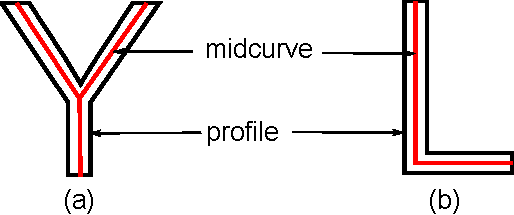
\includegraphics[width=0.45\linewidth]{images/midcurveexamples_1.pdf} 
\caption{Examples of Midcurves}
\label{fig_midcruveexamples}
\end{figure}

%%\bigskip

Figure~\ref{fig_midcruveexamples} shows two examples. Figure~\ref{fig_midcruveexamples}a shows a ``Y'' profile, with its midcurve whereas Figure~\ref{fig_midcruveexamples}b shows a ``L'' profile with its midcurve. Note that, both midcurves are one dimension less and lie midway of the respective profiles.

%%Some representative usages are:
%%\begin{itemize}
%%[noitemsep,topsep=2pt,parsep=2pt,partopsep=2pt,leftmargin=*]
%%\item \textbf{Midsurface}: For Sweep based volumes, Midsurface is nothing but  sweeping of the Midcuves of the Sketch
%%
%%\raisebox{-.9\height}{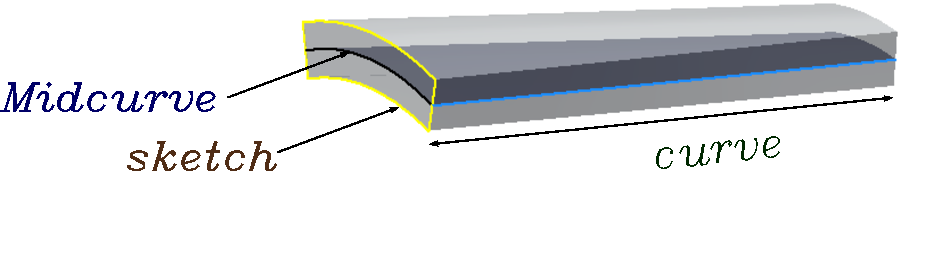
\includegraphics[width=0.5\linewidth]{images/MidsurfSmallProfile.pdf}}
%%
%%\item \textbf{Pattern Matching}: Instead of finding similarity between 2D profiles, it is easier to do the same with Midcurves.
%%
%%\item \textbf{Shape Retrieval}: For retrieving particular 2D shape from the database, Midcurve can be used as signature/meta-data, instead of string/tag based, making selection more deterministic.
%%\end{itemize}

Most of the midsurface generation approaches reviewed in Chapter~\ref{ch:Survey} in Section~\ref{sec:survey:observationsformal} are applicable to midcurve generation as well. Only difference is, instead of a 3D solid model as input for midsurface generation, a 2D profile is the input for midcurve generation. Approaches such as Medial Axis Transform (MAT),  Chordal Axis Transform (CAT), Thinning etc. are used to compute, a generic curve form, known as medial curves. Midcurve is one specialization of the medial curve. Figure~\ref{fig:litsurvey:midcurve}b had shown midcurve output where spurious branches have been replaced by two extensions forming a continuous line, thus mimicking the original shape.

Ramanathan~\cite{Ramanathan2004} states that no formal definition exists for either midcurve or midsurface. He attempted to define midsurface semi-formally as seen in Definition~\ref{def:midsram}. Similarly midcurve can also be defined as:

\begin{mydef}\label{def:midcurve}
Midcurve is an aggregation of curve segments (where each segment corresponds to a pair of nonadjacent edges in the object that are closest to each other) that form a closed and connected set and that satisfy homotopy
\end{mydef}

Review of the reported approaches of computing medial curves is presented in Chapter~\ref{ch:Survey} in Section~\ref{sec:survey:observationsformal}. 
%%
%%Following is summary of some of the salient observations:
%%\begin{itemize}[noitemsep,topsep=2pt,parsep=2pt,partopsep=2pt]
%%	\item Biggest strength of formal approaches like MAT is that it can be computed of any shape, thick or thin. Being formally defined, the converse or reversal process, meaning ``given a MAT compute the original shape'', is possible.
%%	\item Major drawback of MAT, Thinning methods is that it creates unnecessary branches and its shape is smaller than the original corresponding faces.
%%	\item  MAT based approaches also suffer from robustness problem. A slight change in base geometry forces re-computation of MAT and the results could very well be different than the original.
%%	\item Although MAT approaches have been around for decades and are fairly mature, its usage in midcurve generation is still very complex and difficult to ensure appropriate topology.
%%	\item The major limitation of CAT approach is that mesh has to be generated beforehand. Creating constrained, single layer meshes on complicated 2D profiles are, at times, difficult.
%%	\item Thinning approaches are based on split events of the straight line skeleton gives counter-intuitive results if the polygon contains sharp reflex vertices.
%%	\item In Parametric approach, the two input curves or surfaces may not be in one-to-one form. In such cases maintaining continuity can be challenging.
%%	\item Quality of surface generated by parametric approach depends on the sampling done to compute the midpoints.
%%\item Midcurve by profile decomposition approach is not used widely. The decomposition can result in large number of redundant sub-shapes making it ineffective and unstable for further processing.
%%\end{itemize}
%%
It suggests to avoid formal methods such as MAT, CAD, Thinning and Parametric, for computing midcurve as they need heavy post-processing to remove unwanted curves. The heuristic method of decomposition, which has been error prone and inefficient so far, appears promising in case of profile decomposition if enhancements can be proposed.

Following section takes a closer look at some of the existing profile decomposition approaches. After that, existing midcurve generation approaches based on profile decomposition are also reviewed.


\subsection{Related Work}

Many approaches assume the input profile to be of simple polygon type, meaning, all the profile curves are linear and non-intersecting. The polygonal profile is assumed to be a set of connected lines end to end and closing the loop.

Keil~\cite{Keil94} presented an approach based on convex partitioning, i.e. partitioning polygon at concave vertices, with an intent of making sub-polygons, convex. Figure~\ref{fig_keil} shows how his approach finds all possible ways to remove concavity of vertices and then takes the one that requires fewest diagonals.

Lien et. al.~\cite{Lien2004} decomposed polygons 'approximately' based on iterative removal of the most significant non-convex feature. 

Bayazit~\cite{Bayazit} presented a polygon decomposition method based on Concave (Reflex) angle partitioning. Figure~\ref{fig_bayazit} shows the partitioning at specific concave vertices. Although the output was far better than if usual meshing had been employed, the drawback was it left out some corner cases giving more than necessary divisions.

%%\bigskip

	\begin{figure}[!h]
	\centering     %%% not \center
	\subfloat[Keil~\cite{Keil94}]{\label{fig_keil}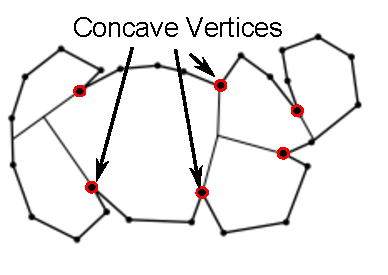
\includegraphics[width=0.4\linewidth]{images/keilwnames.pdf}} \quad
	\subfloat[Bayazit~\cite{Bayazit}]{\label{fig_bayazit}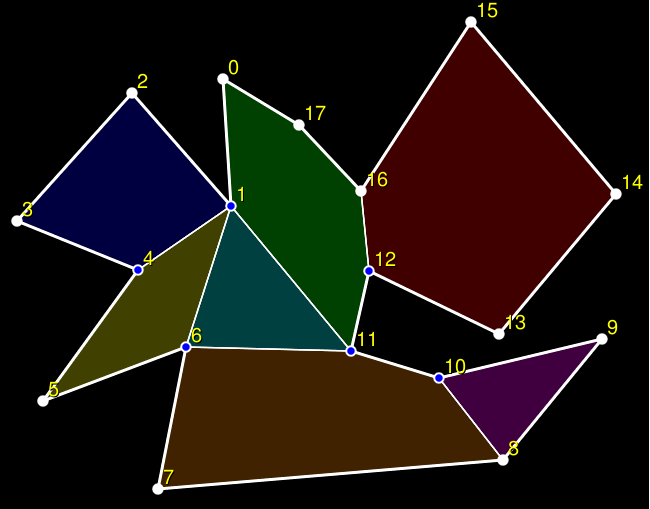
\includegraphics[width=0.4\linewidth]{images/bayazit}}
	\caption{Polygon Decomposition Methods} %%%%%%%% ADD (\{citeYogeshIITG2014}) LATER
	\label{fig:litsurvey:polydecomp}
	\end{figure}
	
%%\bigskip

%%Below is the summary of some of these relevant profile decomposition approaches:
%%
%%\csvreader[longtable=|p{0.17\linewidth}|p{0.11\linewidth}|p{0.15\linewidth}|p{0.2\linewidth}|p{0.17\linewidth}|p{0.17\linewidth}|,
%%    table head=\toprule \bfseries Author & \bfseries Input& \bfseries  Method & \bfseries  Approach& \bfseries  Advantages& \bfseries  Limitations \\ \midrule \endhead,% \bottomrule \endfoot,
%%  late after last line=\\\bottomrule,
%%  before reading={\catcode`\#=12},after reading={\catcode`\#=6},    
%%    late after line=\\\hline]%
%%{litsurvey_polydecomp.csv}{Author=\Author, Input=\Input, Method=\Method, Approach=\Approach, Advantages=\Advantages ,Limitations=\Limitations}%
%%{\Author  & \Input&  \Method &\Approach & \Advantages & \Limitations}%
%%
%%Thus, review of the approaches suggests that the polygon decomposition rules depend on the application context, accuracy, characteristics  and aspect ratio of the sub-polygons. Judicious selection of these parameters will decide the applicability to the problem being solved.
%%
%%Following are some of the midcurve generation approaches based on profile decomposition:
%%
%%% Choi~\cite{Choi1997} subdivided the planar region with holes into smaller simply connected planar sub regions that overlap only at the joints where subdivision occurs. Approximated medials based on Bezier-Bernstein curves are computed for individual sub-regions. 
%%% Decomposition of planar shapes  into regular (non-intersecting) and singular (intersecting regions) and its application to skeletonization has been widely researched~\cite{Rocha99} as well.
%%% 
Rocha~\cite{Rocha98}~\cite{Rocha99} presented skeletonization approach for images which primarily worked on vertices. Figure~\ref{fig_rocha} shows how the sub-shapes computed mid-segments which were joined at the connections. Although this approach could address many shapes, it lacked comprehensive coverage and did not do very well for simple joints like T and L

%%\bigskip

\begin{figure}[h]
\centering 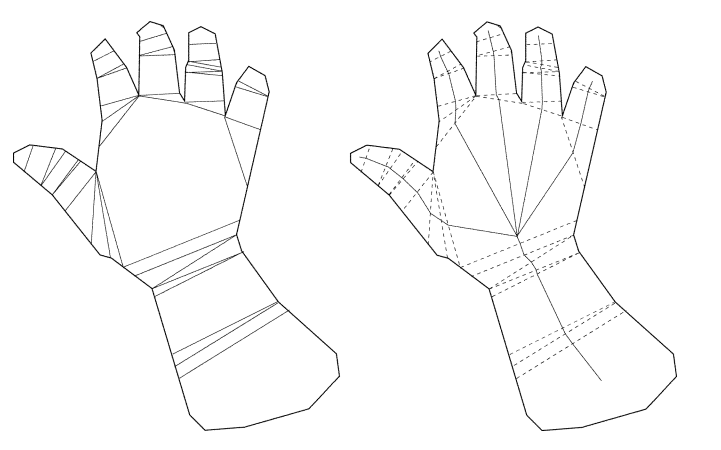
\includegraphics[width=0.5\linewidth]{images/rocha} 
\caption{Midcurve Computation after Polygon Decomposition}
\label{fig_rocha}
\end{figure}

%%\bigskip

%Bag~\cite{Bag2011} computed mid-segments for character image which preserve the local characteristics.
% 
% Below is the summary of the relevant midcurve computation approaches:
% 
%\csvreader[longtable=|p{0.17\linewidth}|p{0.11\linewidth}|p{0.2\linewidth}|p{0.2\linewidth}|p{0.17\linewidth}|p{0.17\linewidth}|,
%    table head=\toprule \bfseries Author & \bfseries Input& \bfseries  Medial& \bfseries  Approach& \bfseries  Advantages& \bfseries  Limitations \\ \midrule \endhead,% \bottomrule \endfoot,
%  late after last line=\\\bottomrule,
%  before reading={\catcode`\#=12},after reading={\catcode`\#=6},    
%    late after line=\\\hline]%
%{litsurvey_midcurvedecomp2d.csv}{Author=\Author, Input=\Input, Method=\Method, Approach=\Approach, Advantages=\Advantages ,Limitations=\Limitations}%
%{\Author  & \Input&  \Method &\Approach & \Advantages & \Limitations}%
%
%\subsubsection{Observations on Midcurve by 2D Decomposition Approaches}

Review of the approaches suggests that the polygon decomposition rules are needed to take into account the application context, accuracy, characteristics  and aspect ratio of the sub-polygons. For the present research work, the midcurve generation needs primitive shaped, thin sub-polygons. Non-primitive, skewed shapes would result in inappropriate midcurves.

Following section proposes midcurve computation approach based on profile decomposition. % method which has improved an existing approach by Bayazit~\cite{Bayazit} to suit the characteristics of sub-polygons needed for computation of midcurve.